%%%%%%%%%%%%%%%%%%%%%%%%%%%%%%%%%%%%%%%%%%%%%%%%%%%%%%%%%%%%%%%%%%%%%%%%%%%%%%%
%  Physlib: a community-run library of formalized physics
%  Joseph Tooby-Smith -- ICARM, 2026
%
%  Same style and preamble as ../Sussex2026/Sussex2026.tex.
%
%  STYLE.  Palette is the one from ../Sussex2025.html and ../UCL2026.html:
%  teal, copper, slate.  The furniture is print, not web -- square corners,
%  hairline rules, no shadows, no rounded "cards", no pill badges, and no
%  decorative icons.  A block is marked by a rule above it and a letterspaced
%  label, the way a table or a sidebar is marked in a book.  The only icons
%  in the deck are the GitHub glyphs on the repository badges, where they
%  are doing a job.
%
%  Compile with: pdflatex Pittsburg2026.tex   (run 3x -- the .nav drives the
%  foot rule, and the frames are fragile)
%%%%%%%%%%%%%%%%%%%%%%%%%%%%%%%%%%%%%%%%%%%%%%%%%%%%%%%%%%%%%%%%%%%%%%%%%%%%%%%
\documentclass[aspectratio=169,10pt]{beamer}

\usepackage[T1]{fontenc}
\usepackage[utf8]{inputenc}
\usepackage[sfdefault]{FiraSans}
% Fira Mono for \ttfamily: it matches Fira Sans, and unlike cmtt it has a
% real bold -- T1/cmtt/bx does not exist, so \bfseries on the mono labels
% was silently falling back to regular weight.
\usepackage[scaled=0.88]{FiraMono}
\usefonttheme[onlymath]{serif}
\usepackage{amsmath,amssymb}
\usepackage{microtype}
\usepackage{tikz}
\usepackage{graphicx}
\usepackage{listings}
\usepackage{fontawesome5}
\usepackage[most]{tcolorbox}
\setlength{\fboxrule}{0.6pt}
\setlength{\fboxsep}{0pt}
\usetikzlibrary{calc,positioning,arrows.meta}

\graphicspath{{../Images/}{Images/}}

\hypersetup{
  pdftitle={Physlib: a community-run library of formalized physics},
  pdfauthor={Joseph Tooby-Smith},
  pdfsubject={Formalisation, Lean, Physlib},
  pdfkeywords={Lean, Physlib, Mathlib, formalisation, AI},
  colorlinks=false, pdfborder={0 0 0},
}

%%%%%%%%%%%%%%%%%%%%%%%%%%%%%%%%%%%%%%%%%%%%%%%%%%%%%%%%%%%%%%%%%%%%%%%%%%%%%%%
%  PALETTE  (from ../Sussex2025.html, ../UCL2026.html, ../IAMP.html)
%%%%%%%%%%%%%%%%%%%%%%%%%%%%%%%%%%%%%%%%%%%%%%%%%%%%%%%%%%%%%%%%%%%%%%%%%%%%%%%
% Two accents and nothing else: a deep teal and its warm complement.  Every
% colour that carries TEXT is at 4.5:1 or better on the page ground, measured,
% not eyeballed -- the old #27AE60 green (2.73:1) and the base teal (2.84:1)
% were both below the 3:1 floor and both were being used for text.
%
%                        on #F9F9F9   on #2F3B4C
%   jttealink  #246B76      5.80         --        text, links, the turnstile
%   jtcopper   #A8432E      5.69         --        text and marks, warm side
%   jtslate    #2F3B4C     10.78         --        body and headings
%   jtgrey     #5A6471      5.71         --        captions and small print
%   jtteal     #4CA1AF       --         3.80       ON DARK only, and the foot bar
\definecolor{jtteal}  {HTML}{4CA1AF}   % light teal: dark grounds, foot bar, tint
\definecolor{jttealink}{HTML}{246B76}  % teal for text on paper
\definecolor{jtcopper}{HTML}{A8432E}   % the warm complement, text-safe
\definecolor{jtslate} {HTML}{2F3B4C}   % headings, dark ground
\definecolor{jtgrey}  {HTML}{5A6471}   % muted text
\definecolor{jtpaper} {HTML}{F9F9F9}   % page ground
\definecolor{jtmist}  {HTML}{C4E0E5}   % pale teal, used only as a tint

% kept as an alias so older call sites still resolve
\definecolor{jtcopperink}{HTML}{A8432E}
\definecolor{jtrule}     {HTML}{D5DBE1}   % hairlines

% The dark ground of the title, dividers and closing, and the colours that sit
% on it.  Lightening the ground costs contrast, so the muted text and the mark
% colour were lightened with it rather than left to fail:
%
%                        on #3E5063
%   jtondark   #F2F5F7      7.57     title and section text
%   jtondarkm  #B8C6D2      4.76     muted text        (was 3.49 on this ground)
%   jtondarka  #6FC0CC      3.98     rules and marks   (was 2.77 on this ground)
%
% jtground is separate from jtslate on purpose: jtslate is the body-text
% colour on light slides and must stay dark.
\definecolor{jtground}  {HTML}{3E5063}
% A second, deeper ground used ONLY by the Physics 1.0 / 2.0 pair, so they do
% not read as another title slide.  Hue-shifted toward the deck's teal, and
% darker, so every on-dark colour gains contrast rather than losing it:
% text 9.75:1, muted 6.12:1, accent 5.13:1 (vs 7.57 / 4.76 / 3.98 on jtground).
\definecolor{jtgroundalt}{HTML}{27424B}
% A pale warm ground that marks the slides which state a PROBLEM.  Distinct
% enough to be read at a glance, quiet enough not to compete with the dark
% title and divider slides.  Slate on it is 10.2:1.
\definecolor{jtproblembg}{HTML}{FBF3F0}
\definecolor{jtondark}  {HTML}{F2F5F7}
\definecolor{jtondarkm} {HTML}{B8C6D2}
\definecolor{jtondarka} {HTML}{6FC0CC}

%%%%%%%%%%%%%%%%%%%%%%%%%%%%%%%%%%%%%%%%%%%%%%%%%%%%%%%%%%%%%%%%%%%%%%%%%%%%%%%
%  BACKGROUNDS
%  A hairline along the foot shows how far through the deck we are.  Before
%  the .nav exists \inserttotalframenumber is 1, so clamp the fraction or a
%  first pass on a clean tree overflows a TeX dimension.
%%%%%%%%%%%%%%%%%%%%%%%%%%%%%%%%%%%%%%%%%%%%%%%%%%%%%%%%%%%%%%%%%%%%%%%%%%%%%%%
\newcommand{\jtFootRule}[1]{%
  \ifnum\inserttotalframenumber>0\relax
    \pgfmathsetmacro{\jtfrac}{min(1,\insertframenumber/\inserttotalframenumber)}%
  \else
    \def\jtfrac{0}%
  \fi
  \fill[#1] (current page.south west)
    rectangle ([xshift=\jtfrac\paperwidth,yshift=0.055cm]current page.south west);}

\newcommand{\jtBackground}{%
  \begin{tikzpicture}[remember picture,overlay]
    \fill[jtpaper] (current page.south west) rectangle (current page.north east);
    \jtFootRule{jtteal}
  \end{tikzpicture}%
}

\newcommand{\jtBackgroundDark}{%
  \begin{tikzpicture}[remember picture,overlay]
    \fill[jtground] (current page.south west) rectangle (current page.north east);
    \jtFootRule{jtondarka}
  \end{tikzpicture}%
}

% The Physics 1.0 / 2.0 ground.
\newcommand{\jtBackgroundAlt}{%
  \begin{tikzpicture}[remember picture,overlay]
    \fill[jtgroundalt] (current page.south west) rectangle (current page.north east);
    \jtFootRule{jtondarka}
  \end{tikzpicture}%
}

% Problem slides: same furniture, warmer paper.
\newcommand{\jtBackgroundProblem}{%
  \begin{tikzpicture}[remember picture,overlay]
    \fill[jtproblembg] (current page.south west) rectangle (current page.north east);
    \jtFootRule{jtcopper}
  \end{tikzpicture}%
}
% Wrap a frame in this to mark it as stating a problem.
\newenvironment{jtproblem}{%
  \begingroup\setbeamertemplate{background}{\jtBackgroundProblem}%
}{\endgroup}


\setbeamertemplate{background}{\jtBackground}

%%%%%%%%%%%%%%%%%%%%%%%%%%%%%%%%%%%%%%%%%%%%%%%%%%%%%%%%%%%%%%%%%%%%%%%%%%%%%%%
%  TYPE
%    \jtlabel{...}  a small bold lowercase label in the accent colour
%    \jtbody        body text inside a block
%    \jtmeta        captions, attributions, small print
%%%%%%%%%%%%%%%%%%%%%%%%%%%%%%%%%%%%%%%%%%%%%%%%%%%%%%%%%%%%%%%%%%%%%%%%%%%%%%%
% Labels are set lowercase in the mono face, the way an identifier is written
% in source.  Deliberately not letterspaced caps: that, over a rule, on a
% rounded card, is the house style of every generated deck.
\newcommand{\jtlabel}[1]{{\bfseries\fontsize{8.5}{10.5}\selectfont
  \MakeLowercase{#1}}}
% A heading-weight label that keeps its capitals, for the few blocks whose
% label is doing real work rather than just naming a slot.
\newcommand{\jtlabelcap}[1]{{\bfseries\fontsize{11.5}{14}\selectfont #1}}
\newcommand{\jtbody}{\small}
\newcommand{\jtmeta}{\footnotesize}

%%%%%%%%%%%%%%%%%%%%%%%%%%%%%%%%%%%%%%%%%%%%%%%%%%%%%%%%%%%%%%%%%%%%%%%%%%%%%%%
%  BEAMER FURNITURE
%%%%%%%%%%%%%%%%%%%%%%%%%%%%%%%%%%%%%%%%%%%%%%%%%%%%%%%%%%%%%%%%%%%%%%%%%%%%%%%
\setbeamertemplate{navigation symbols}{}
\setbeamersize{text margin left=0.9cm,text margin right=0.9cm}
\setbeamercolor{normal text}{fg=jtslate}
\setbeamercolor{frametitle}{fg=jtslate}
\setbeamerfont{frametitle}{size=\Large,series=\bfseries}
\setbeamertemplate{itemize item}{\raisebox{0.2ex}{\tiny\textbullet}}
\setbeamercolor{itemize item}{fg=jttealink}
\setlength{\parskip}{2pt}
\setlength{\leftmargini}{1.2em}
\setlength{\abovedisplayskip}{4pt}
\setlength{\belowdisplayskip}{2pt}
\setlength{\abovedisplayshortskip}{4pt}
\setlength{\belowdisplayshortskip}{2pt}

% The running section name, reset by \jtpart at each divider.  It sits above
% the frame title as a kicker, the way a running head sits on a book page.
\newcommand{\jtkicker}{}
\newcommand{\jtsetkicker}[1]{\gdef\jtkicker{#1}}

% The turnstile, entailment: "from what has been assumed, this follows".  It
% hangs in the left margin beside every frame title and opens every section
% divider.  It is the one ornament in the deck, and it is the subject's own.
\newcommand{\jtturn}{$\vdash$}

\setbeamertemplate{frametitle}{%
  \vspace*{0.20cm}%
  \begin{minipage}{\dimexpr\paperwidth-1.8cm\relax}
    \raggedright
    {\color{jttealink}\jtturn\hspace{5pt}\jtlabel{\jtkicker}\par}
    \vspace{1pt}
    {\usebeamerfont{frametitle}\usebeamercolor[fg]{frametitle}\insertframetitle\par}
    \vspace{3pt}
    {\color{jtslate}\rule{\linewidth}{0.9pt}}
  \end{minipage}\par\vspace{0.10cm}%
}

\setbeamertemplate{footline}{%
  \hbox{%
    \begin{beamercolorbox}[wd=\paperwidth,ht=2.0ex,dp=3.4ex,%
        leftskip=0.9cm,rightskip=0.9cm]{}%
      {\scriptsize\color{jtgrey}Joseph Tooby-Smith\;\textbullet\;University of Bath}%
      \hfill
      {\scriptsize\color{jtgrey}\insertframenumber}%
    \end{beamercolorbox}}%
}

%%%%%%%%%%%%%%%%%%%%%%%%%%%%%%%%%%%%%%%%%%%%%%%%%%%%%%%%%%%%%%%%%%%%%%%%%%%%%%%
%  BLOCKS
%  No rules at all -- not above a block, not beside one.  A block is a quiet
%  panel: white on the off-white page, or a pale tint for a statement that
%  carries weight.  The accent survives in the label, not in an ornament.
%%%%%%%%%%%%%%%%%%%%%%%%%%%%%%%%%%%%%%%%%%%%%%%%%%%%%%%%%%%%%%%%%%%%%%%%%%%%%%%
\tcbset{
  jtbase/.style={
    enhanced, sharp corners, boxrule=0pt, colback=white,
    left=14pt, right=11pt, top=8pt, bottom=8pt,
    halign=flush left, before skip=5pt, after skip=5pt,
  }
}
% [opts] {accent} {label}  -- label may be empty for an unlabelled block
\newtcolorbox{jtblock}[3][]{jtbase,
  #1,
  before upper={\ifx\relax#3\relax\else{\color{#2}\jtlabel{#3}}\par\vspace{6pt}\fi}}
% same, but the label keeps its capitals and is set to stand out
\newtcolorbox{jtblockcap}[3][]{jtbase,
  #1,
  before upper={\ifx\relax#3\relax\else{\color{#2}\jtlabelcap{#3}}\par\vspace{7pt}\fi}}
% Row variant: every block carrying the same group name (#4) is set to the
% natural height of the tallest one, so a row aligns without a hard-coded
% height that the text can outgrow.  Needs two passes to settle.
\newtcolorbox{jtblockh}[4][]{jtbase, equal height group=#4,
  #1,
  before upper={\ifx\relax#3\relax\else{\color{#2}\jtlabel{#3}}\par\vspace{6pt}\fi}}

% A quiet block on a tinted ground, for a single statement.
\newtcolorbox{jtquote}[2][]{enhanced, sharp corners, boxrule=0pt,
  colback=jtmist!28, left=18pt, right=16pt, top=12pt, bottom=12pt,
  before skip=5pt, after skip=5pt, halign=flush left, #1}

% A named thing, set off by a rule down its left edge.  Used where three or
% four things are being named rather than described.
%   #1 accent  #2 the word  #3 gloss (or {})
\newcommand{\jtstack}[3]{%
  {\color{#1}\fontsize{17}{21}\selectfont\bfseries\raggedright #2\par}
  \ifx\relax#3\relax\else\vspace{5pt}{\jtmeta\color{jtgrey}\raggedright #3\par}\fi}

% One quiet panel naming a single thing -- a row of these reads as separate
% items, where bare stacked words read as a block of text.
% Defined here, not in the frame: \newcommand with an argument inside a frame
% body breaks, because beamer re-scans the body.
\newcommand{\jtrole}[1]{%
  \begin{jtblock}[top=7pt,bottom=7pt,before skip=3pt,after skip=3pt]{jttealink}{}
    {\fontsize{14}{18}\selectfont\bfseries\color{jtslate}#1\strut\par}
  \end{jtblock}}

% A figure set large, with its label beneath.  #1 accent  #2 figure  #3 label
\newcommand{\jtfigure}[3]{%
  {\color{#1}\fontsize{34}{36}\selectfont\bfseries #2\par}
  \vspace{6pt}
  {\color{jtslate}\fontsize{13}{17}\selectfont\bfseries #3\par}}

% The Physics 1.0 and Physics 2.0 tables are a matched pair: same ground,
% same header, same row metrics.  They share this machinery so they cannot
% drift apart.  \jtstate is one state, \jtshift is a state changing.
\newcommand{\jtrowhead}[1]{{\color{jttealink}\jtlabel{#1}\par}\vspace{2pt}}
\newcommand{\jtstate}[2]{%
  \jtrowhead{#1}%
  {\fontsize{15}{20}\selectfont{\color{jtslate}#2}\par}
  \vspace{9pt}}

% before -> after, on the dark ground.  #1 tenet, #2 before, #3 after
\newcommand{\jtshift}[3]{%
  \jtrowhead{#1}%
  {\fontsize{15}{20}\selectfont
    {\color{jtgrey}#2}\quad{\color{jtcopper}$\rightarrow$}\quad
    {\color{jtslate}\bfseries #3}\par}
  \vspace{9pt}}

% Numbered points.  The numeral hangs in the accent colour.
\newcommand{\jtnum}[3]{{\fontsize{16}{21}\selectfont
  \hangindent=1.6em \hangafter=1
  \makebox[1.6em][l]{\color{#1}\bfseries#2}{\color{jtslate}#3}\par}}
\newcommand{\jtnumxs}[3]{{\fontsize{12.5}{17}\selectfont
  \hangindent=1.6em \hangafter=1
  \makebox[1.6em][l]{\color{#1}\bfseries#2}{\color{jtslate}#3}\par}}
\newcommand{\jtnumsm}[3]{{\fontsize{14}{19}\selectfont
  \hangindent=1.6em \hangafter=1
  \makebox[1.6em][l]{\color{#1}\bfseries#2}{\color{jtslate}#3}\par}}

%%%%%%%%%%%%%%%%%%%%%%%%%%%%%%%%%%%%%%%%%%%%%%%%%%%%%%%%%%%%%%%%%%%%%%%%%%%%%%%
%  REPOSITORY BADGE
%  Deliberately GitHub-like -- it is quoting a page the audience knows -- so
%  this is the one place in the deck that keeps its icons.
%  #1 owner  #2 repo  #3 url  #4 blurb  #5 stats
%%%%%%%%%%%%%%%%%%%%%%%%%%%%%%%%%%%%%%%%%%%%%%%%%%%%%%%%%%%%%%%%%%%%%%%%%%%%%%%
\newtcolorbox{jtbadge}{enhanced, nobeforeafter, box align=center,
  sharp corners, width=4.4cm, height=4.55cm, valign=top, halign=flush left,
  colback=white, colframe=jtrule, boxrule=0.9pt,
  left=11pt,right=11pt,top=10pt,bottom=10pt}
\newcommand{\jtrepo}[5]{%
  \begin{jtbadge}
    {\color{jtgrey}\fontsize{15}{15}\selectfont\faIcon{github}}\par
    \vspace{7pt}
    % \href takes a box, not a paragraph, so the two lines go in a \parbox.
    \href{#3}{\parbox{\linewidth}{\raggedright
      {\fontsize{6.8}{8}\selectfont\color{jtgrey}#1\,/}\\[1.5pt]
      {\fontsize{14}{16}\selectfont\bfseries\color{jtslate}#2}}}
    \par\vspace{6pt}
    {\fontsize{7.6}{9.6}\selectfont\color{jtgrey}\raggedright #4\par}
    \vfill
    {\color{jtrule}\rule{\linewidth}{0.7pt}}\par\vspace{4pt}
    {\fontsize{6.8}{9}\selectfont\color{jtgrey}#5\par}
  \end{jtbadge}}

%%%%%%%%%%%%%%%%%%%%%%%%%%%%%%%%%%%%%%%%%%%%%%%%%%%%%%%%%%%%%%%%%%%%%%%%%%%%%%%
%  WIDE REPOSITORY CARD
%  The full-width form used in ../CACS2026 and ../BathSeptember26, for when a
%  single repository is the point of the slide.
%  #1 owner #2 repo #3 url #4 blurb #5 stars #6 forks #7 contributors #8 year
%%%%%%%%%%%%%%%%%%%%%%%%%%%%%%%%%%%%%%%%%%%%%%%%%%%%%%%%%%%%%%%%%%%%%%%%%%%%%%%
\newcommand{\jtrepowide}[8]{%
  \begin{tcolorbox}[enhanced, sharp corners, width=0.94\textwidth,
      colback=white, colframe=jtrule, boxrule=0.9pt,
      left=18pt,right=18pt,top=13pt,bottom=13pt]
    \begin{minipage}[c]{0.09\textwidth}
      {\color{jtgrey}\fontsize{26}{26}\selectfont\faIcon{github}}
    \end{minipage}\hfill
    \begin{minipage}[c]{0.72\textwidth}
      \href{#3}{{\Large\bfseries\color{jtslate}#1\,/\,#2}}\\[4pt]
      {\jtbody\color{jtgrey}\raggedright #4\par}
    \end{minipage}\hfill
    \begin{minipage}[c]{0.15\textwidth}
      \raggedleft
      {\color{jtgrey}\jtlabel{public}}\\[3pt]
      {\color{jtgrey}\jtlabel{Lean 4}}
    \end{minipage}

    \vspace{11pt}{\color{jtrule}\rule{\linewidth}{0.8pt}}\vspace{7pt}

    {\jtmeta\color{jtgrey}%
      \faIcon{star}\;\textbf{#5} stars
      \hspace{1.0em}\faIcon{code-branch}\;\textbf{#6} forks
      \hspace{1.0em}\faIcon{users}\;\textbf{#7} contributors
      \hspace{1.0em}\faIcon{clock}\;started #8}
  \end{tcolorbox}}

%%%%%%%%%%%%%%%%%%%%%%%%%%%%%%%%%%%%%%%%%%%%%%%%%%%%%%%%%%%%%%%%%%%%%%%%%%%%%%%
%  SECTION DIVIDERS
%  A contents list on a slate ground, with the section we are entering picked
%  out.  Edit the three names here and the change lands on every divider.
%%%%%%%%%%%%%%%%%%%%%%%%%%%%%%%%%%%%%%%%%%%%%%%%%%%%%%%%%%%%%%%%%%%%%%%%%%%%%%%
\newcommand{\jtsecA}{The formalization landscape}
\newcommand{\jtsecB}{Physlib: the details}
\newcommand{\jtsecC}{How to contribute?}

% #1 = section being entered, #2 = this row's number, #3 = this row's name
\newcommand{\jtrow}[3]{%
  \ifnum#1=#2\relax
    \rlap{\hspace*{-0.85cm}{\color{jtondarka}\rule[0.18ex]{0.5cm}{1.4pt}}}%
    {\color{jtondark}\bfseries #3}%
  \else
    {\color{jtondarkm}#3}%
  \fi\par\vspace{5pt}}

% #1 = section number, #2 = section title
\newcommand{\jtpartbody}[2]{%
  \vfill
  \begin{columns}[T,onlytextwidth]
    \begin{column}{0.56\textwidth}
      {\color{jtondarka}\Large\jtturn}\par
      \vspace{12pt}
      {\color{jtondarkm}\jtlabel{section #1 of 3}\par}
      \vspace{10pt}
      {\color{jtondark}\fontsize{27}{32}\selectfont\bfseries\raggedright #2\par}
    \end{column}
    \begin{column}{0.38\textwidth}
      \vspace{6pt}
      {\jtmeta
        \jtrow{#1}{1}{\jtsecA}%
        \jtrow{#1}{2}{\jtsecB}%
        \jtrow{#1}{3}{\jtsecC}}
    \end{column}
  \end{columns}
  \vfill}

% A divider frame: slate ground, no footline.  #1 number, #2 title, #3 kicker
% for the frames that follow.
\newenvironment{jtsection}[3]{%
  \jtsetkicker{#3}%
  \begingroup
  \setbeamertemplate{background}{\jtBackgroundDark}%
  \setbeamertemplate{footline}{}%
  \begin{frame}[plain]
  \jtpartbody{#1}{#2}%
}{%
  \end{frame}
  \endgroup
}

%%%%%%%%%%%%%%%%%%%%%%%%%%%%%%%%%%%%%%%%%%%%%%%%%%%%%%%%%%%%%%%%%%%%%%%%%%%%%%%
%  LEAN LISTINGS  (ASCII-only source, so pdflatex stays happy)
%%%%%%%%%%%%%%%%%%%%%%%%%%%%%%%%%%%%%%%%%%%%%%%%%%%%%%%%%%%%%%%%%%%%%%%%%%%%%%%
\lstdefinelanguage{lean}{
  morekeywords={theorem,lemma,def,abbrev,example,structure,instance,class,where,
    by,fun,have,show,from,let,match,with,namespace,end,open,variable,
    intro,exact,apply,simp,rfl,ring,unfold,positivity,sorry,Type,Prop,Sort,
    induction,rw,at,
    inductive,cases,Empty,Ne,Nat},
  sensitive=true,
  morecomment=[l]{--},
  morecomment=[s]{/-}{-/},
  morestring=[b]",
}
\lstset{
  language=lean,
  basicstyle=\ttfamily\small\color{jtslate},
  keywordstyle=\bfseries\color{jttealink},
  commentstyle=\itshape\color{jtgrey},
  showstringspaces=false,
  columns=fullflexible,
  breaklines=false,
  aboveskip=1pt, belowskip=1pt,
}

%%%%%%%%%%%%%%%%%%%%%%%%%%%%%%%%%%%%%%%%%%%%%%%%%%%%%%%%%%%%%%%%%%%%%%%%%%%%%%%
%%%%%%%%%%%%%%%%%%%%%%%%%%%%%%%%%%%%%%%%%%%%%%%%%%%%%%%%%%%%%%%%%%%%%%%%%%%%%%%
%  PITTSBURGH ADDITIONS
%  Colour carries one meaning through the talk: copper is fast and furious
%  formalization, teal is the trusted corpus.
%%%%%%%%%%%%%%%%%%%%%%%%%%%%%%%%%%%%%%%%%%%%%%%%%%%%%%%%%%%%%%%%%%%%%%%%%%%%%%%
% Same as jtblockcap, but every block in group #4 gets the same height.
\newtcolorbox{jtblockcaph}[4][]{jtbase, equal height group=#4,
  #1,
  before upper={\ifx\relax#3\relax\else{\color{#2}\jtlabelcap{#3}}\par\vspace{7pt}\fi}}

% A core library (solid teal) inside a fuzzy copper halo of fast and furious
% projects.  The halo is many faint copper disks stacked, so it is densest at
% the core and fades out to nothing.  With an empty halo label no halo is
% drawn, but its space is kept so a row of these still lines up.
%   #1 core radius   #2 core label   #3 halo label (or {})
%   #4 core label font   #5 halo label font
\newcommand{\jthalo}[5]{%
  \begin{tikzpicture}[baseline=(jtcore.base)]
    \path (0,0) circle ({2.02*#1});
    \ifx\relax#3\relax\else
      \foreach \i in {0,...,29}
        \fill[jtcopper,opacity=0.017] (0,0) circle ({#1*(1+0.034*\i)});
      \node[text=jtcopper,font=#5,align=center] at (0,{1.5*#1}) {#3};
    \fi
    \fill[jttealink] (0,0) circle (#1);
    \node[text=white,font=#4,align=center] (jtcore) at (0,0) {#2};
  \end{tikzpicture}}

% Number of people on the Zulip.
\newcommand{\jtzulip}{340}

% An activity with a one-line example beneath it.  Blocks sharing a group
% name (#1) get the same height, so a row lines up when an example wraps.
%   #1 row group  #2 activity  #3 example
\newcommand{\jtroleex}[3]{%
  \begin{jtblockh}[top=7pt,bottom=8pt,before skip=3pt,after skip=3pt]{jttealink}{}{#1}
    {\fontsize{14}{18}\selectfont\bfseries\color{jtslate}#2\strut\par}
    \vspace{1pt}
    {\jtmeta\color{jtgrey}\raggedright #3\par}
  \end{jtblockh}}

% One figure on the repository card: icon, number, label.
\newcommand{\jtcardstat}[3]{%
  {\color{jtgrey}\fontsize{13}{13}\selectfont\faIcon{#1}}\hspace{6pt}%
  {\color{jtslate}\fontsize{22}{24}\selectfont\bfseries #2}\par\vspace{3pt}
  {\jtmeta\color{jtgrey}#3\par}}

%%%%%%%%%%%%%%%%%%%%%%%%%%%%%%%%%%%%%%%%%%%%%%%%%%%%%%%%%%%%%%%%%%%%%%%%%%%%%%%
% TODO: set the talk date here; it is used by \date and the title slide.
\newcommand{\jttalkdate}{November 2026}

\title{Physlib}
\author{Joseph Tooby-Smith}
\date{\jttalkdate}

\begin{document}

%%%%%%%%%%%%%%%%%%%%%%%%%%%%%%%%%%%%%%%%%%%%%%%%%%%%%%%%%%%%%%%%%%%%%%%%%%%%%%%
%    TITLE
%%%%%%%%%%%%%%%%%%%%%%%%%%%%%%%%%%%%%%%%%%%%%%%%%%%%%%%%%%%%%%%%%%%%%%%%%%%%%%%
{
\setbeamertemplate{background}{\jtBackgroundDark}
\setbeamertemplate{footline}{}
\begin{frame}[plain]
  \vfill
  \begin{columns}[T,onlytextwidth]
    \begin{column}{0.97\textwidth}
      {\color{jtondarka}\rule{3.2cm}{2pt}}\par
      \vspace{14pt}
      {\color{jtondarkm}\bfseries\fontsize{8.5}{10.5}\selectfont
        ICARM \;\textbullet\; \jttalkdate\par}
      \vspace{14pt}
      {\color{jtondark}\fontsize{46}{52}\selectfont\bfseries Physlib\par}
      \vspace{10pt}
      {\color{jtondarkm}\fontsize{17}{22}\selectfont
        A community-run library of formalized physics\par}
      \vspace{16pt}
      {\color{jtondarkm}\rule{\linewidth}{0.5pt}}\par
      \vspace{12pt}
      {\color{jtondark}\fontsize{13}{16}\selectfont\bfseries Joseph Tooby-Smith\par}
      \vspace{4pt}
      {\color{jtondarkm}\jtmeta University of Bath\par}
      \vspace{14pt}
      {\color{jtondarkm}\jtmeta
        \href{https://github.com/leanprover-community/physlib}{%
          \color{jtondarkm}github.com/leanprover-community/physlib}
        \qquad
        \href{https://josephtoobysmith.com/}{%
          \color{jtondarkm}josephtoobysmith.com}\par}
    \end{column}
  \end{columns}
  \vfill
\end{frame}
}

%%%%%%%%%%%%%%%%%%%%%%%%%%%%%%%%%%%%%%%%%%%%%%%%%%%%%%%%%%%%%%%%%%%%%%%%%%%%%%%
%    OVERVIEW  (the section names come from \jtsecA--\jtsecC, so they stay in
%    step with the dividers)
%%%%%%%%%%%%%%%%%%%%%%%%%%%%%%%%%%%%%%%%%%%%%%%%%%%%%%%%%%%%%%%%%%%%%%%%%%%%%%%
\jtsetkicker{Physlib}
\begin{frame}{Overview}
  \vfill
  \begin{minipage}{0.94\textwidth}
    \raggedright
    \jtnum{jttealink}{1}{\jtsecA}
    \vspace{16pt}
    \jtnum{jttealink}{2}{\jtsecB}
    \vspace{16pt}
    \jtnum{jttealink}{3}{\jtsecC}
  \end{minipage}
  \vfill
\end{frame}

%%%%%%%%%%%%%%%%%%%%%%%%%%%%%%%%%%%%%%%%%%%%%%%%%%%%%%%%%%%%%%%%%%%%%%%%%%%%%%%
%    SECTION 1 -- THE FORMALIZATION LANDSCAPE
%%%%%%%%%%%%%%%%%%%%%%%%%%%%%%%%%%%%%%%%%%%%%%%%%%%%%%%%%%%%%%%%%%%%%%%%%%%%%%%
\begin{jtsection}{1}{\jtsecA}{The formalization landscape}
\end{jtsection}

%%%%%%%%%%%%%%%%%%%%%%%%%%%%%%%%%%%%%%%%%%%%%%%%%%%%%%%%%%%%%%%%%%%%%%%%%%%%%%%
%  1.1  A SHIFT IN ACTIVITIES  (then -> now)
%%%%%%%%%%%%%%%%%%%%%%%%%%%%%%%%%%%%%%%%%%%%%%%%%%%%%%%%%%%%%%%%%%%%%%%%%%%%%%%
\begin{frame}{A shift in activities}
  \vfill
  \begin{center}
  \begin{minipage}{0.72\textwidth}
    \begin{jtblockcap}[top=14pt,bottom=14pt]{jttealink}{Back in 2023, within Lean}
      {\fontsize{17}{24}\selectfont\color{jtslate}%
        Formalization was synonymous with building a
        {\bfseries community run standard library} (corpus of
        knowledge), {\bfseries Mathlib}\ldots\par}
    \end{jtblockcap}
  \end{minipage}
  \end{center}
  \vfill
  {\jtmeta\color{jtgrey}(By standard library, or corpus of knowledge, I mean
  a high quality collection of results.)\par}
\end{frame}

%%%%%%%%%%%%%%%%%%%%%%%%%%%%%%%%%%%%%%%%%%%%%%%%%%%%%%%%%%%%%%%%%%%%%%%%%%%%%%%
%  1.2  SINCE THEN  (one line forking in two)
%%%%%%%%%%%%%%%%%%%%%%%%%%%%%%%%%%%%%%%%%%%%%%%%%%%%%%%%%%%%%%%%%%%%%%%%%%%%%%%
\begin{frame}{Since then\ldots}
  \vfill
  \begin{center}
  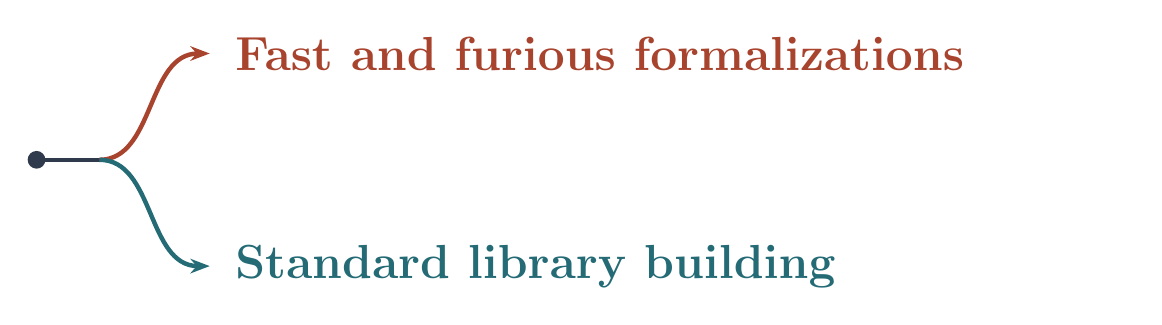
\begin{tikzpicture}
    \fill[jtslate] (0,0) circle (3.2pt);
    \draw[jtslate,line width=1.6pt] (0,0) -- (0.8,0);
    \draw[jtcopper,line width=1.6pt,-{Stealth[length=7pt]}]
      (0.8,0) .. controls (1.5,0) and (1.4,1.35) .. (2.2,1.35);
    \draw[jttealink,line width=1.6pt,-{Stealth[length=7pt]}]
      (0.8,0) .. controls (1.5,0) and (1.4,-1.35) .. (2.2,-1.35);
    \node[anchor=west,text=jtcopper,text width=11.3cm,
          font=\fontsize{17}{21}\selectfont\bfseries] at (2.4,1.35)
      {Fast and furious formalizations};
    \node[anchor=west,text=jttealink,text width=11.3cm,
          font=\fontsize{17}{21}\selectfont\bfseries] at (2.4,-1.35)
      {Standard library building};
  \end{tikzpicture}
  \end{center}
  \vfill
\end{frame}

%%%%%%%%%%%%%%%%%%%%%%%%%%%%%%%%%%%%%%%%%%%%%%%%%%%%%%%%%%%%%%%%%%%%%%%%%%%%%%%
%  1.3  MUTUALLY REINFORCING, WITH DIFFERENT PURPOSES
%%%%%%%%%%%%%%%%%%%%%%%%%%%%%%%%%%%%%%%%%%%%%%%%%%%%%%%%%%%%%%%%%%%%%%%%%%%%%%%
\begin{frame}{These are mutually reinforcing, with different purposes}
  \vfill
  % The fork from "Since then", now ending on the two panels,
  % stacked.  The fork is centred on the gap between the panels, and each
  % branch lands on the middle of its panel's left edge.
  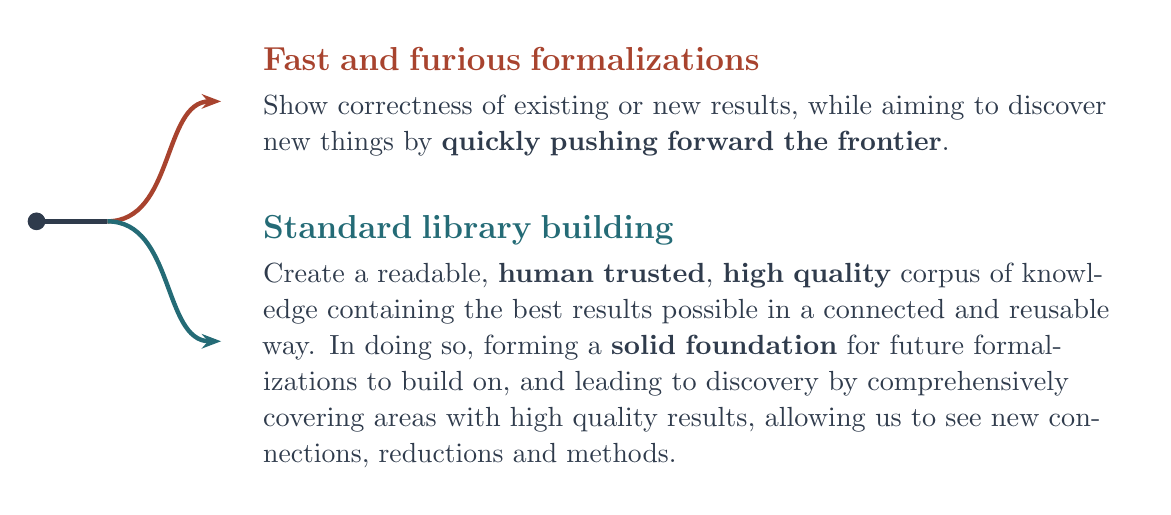
\begin{tikzpicture}[
      panel/.style={fill=white,anchor=north west,align=left,
        inner xsep=12pt,inner ysep=7pt,text width=10.75cm},
      branch/.style={line width=1.6pt,-{Stealth[length=7pt]},shorten >=3pt}]
    \node[panel] (ff) at (2.45,0) {%
      {\color{jtcopper}\fontsize{13}{15}\selectfont\bfseries
        Fast and furious formalizations\par}
      \vspace{3pt}
      {\fontsize{10}{13}\selectfont\color{jtslate}%
        Show correctness of existing or new results, while aiming to
        discover new things by {\bfseries quickly pushing forward the
        frontier}.\par}};
    \node[panel,below=7pt of ff.south west,anchor=north west] (tc) {%
      {\color{jttealink}\fontsize{13}{15}\selectfont\bfseries
        Standard library building\par}
      \vspace{3pt}
      {\fontsize{10}{13}\selectfont\color{jtslate}%
        Create a readable, {\bfseries human trusted}, {\bfseries high
        quality} corpus of knowledge containing the best results possible
        in a connected and reusable way. In doing so, forming a {\bfseries solid foundation} for future
        formalizations to build on, and leading to discovery by
        comprehensively covering areas with high quality results, allowing
        us to see new connections, reductions and methods.\par}};
    \coordinate (mid) at ($(ff.west)!0.5!(tc.west)$);
    \coordinate (root)  at ($(mid)+(-2.45,0)$);
    \coordinate (split) at ($(mid)+(-1.55,0)$);
    \fill[jtslate] (root) circle (3.2pt);
    \draw[jtslate,line width=1.6pt] (root) -- (split);
    \draw[branch,jtcopper]  (split) to[out=0,in=180] (ff.west);
    \draw[branch,jttealink] (split) to[out=0,in=180] (tc.west);
  \end{tikzpicture}
  \vfill
\end{frame}

%%%%%%%%%%%%%%%%%%%%%%%%%%%%%%%%%%%%%%%%%%%%%%%%%%%%%%%%%%%%%%%%%%%%%%%%%%%%%%%
%  1.3a  AN ANALOGY
%  The picture is forest.tex, generated by forest.py (python3 forest.py >
%  forest.tex).  Colours keep their meaning: copper footpaths are fast and
%  furious formalization, the teal road is standard library building.
%%%%%%%%%%%%%%%%%%%%%%%%%%%%%%%%%%%%%%%%%%%%%%%%%%%%%%%%%%%%%%%%%%%%%%%%%%%%%%%
\begin{frame}{An analogy}
  \vfill
  \begin{columns}[c,onlytextwidth]
    \begin{column}{0.55\textwidth}
      \centering
      \resizebox{\linewidth}{!}{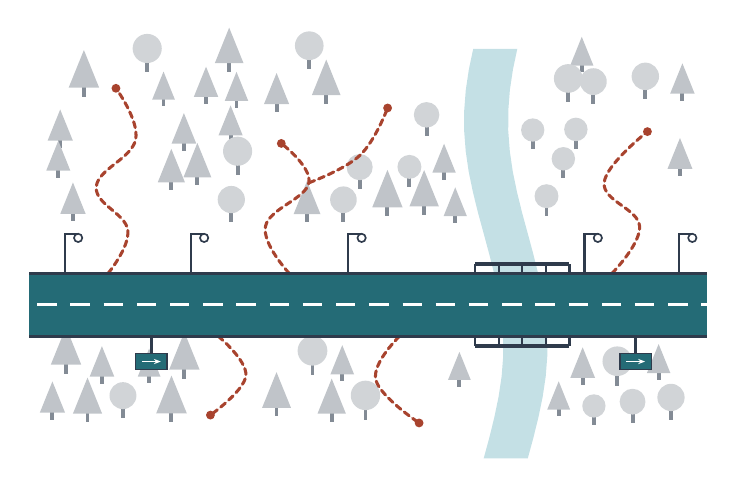
\begin{tikzpicture}[x=1cm,y=1cm]
  \path (0,0) rectangle (8.60,5.20);
  \fill[jtmist] (5.770,0.000) -- (5.841,0.260) -- (5.905,0.520) -- (5.959,0.780) -- (5.998,1.040) -- (6.018,1.300) -- (6.017,1.560) -- (5.997,1.820) -- (5.958,2.080) -- (5.904,2.340) -- (5.839,2.600) -- (5.769,2.860) -- (5.698,3.120) -- (5.634,3.380) -- (5.580,3.640) -- (5.542,3.900) -- (5.522,4.160) -- (5.523,4.420) -- (5.543,4.680) -- (5.582,4.940) -- (5.637,5.200) -- (6.197,5.200) -- (6.142,4.940) -- (6.103,4.680) -- (6.083,4.420) -- (6.082,4.160) -- (6.102,3.900) -- (6.140,3.640) -- (6.194,3.380) -- (6.258,3.120) -- (6.329,2.860) -- (6.399,2.600) -- (6.464,2.340) -- (6.518,2.080) -- (6.557,1.820) -- (6.577,1.560) -- (6.578,1.300) -- (6.558,1.040) -- (6.519,0.780) -- (6.465,0.520) -- (6.401,0.260) -- (6.330,0.000) -- cycle;
  \fill[jtgrey!75] (3.530,4.941) rectangle ++(0.05,0.172);
  \fill[jtgrey!28] (3.555,5.241) circle (0.182);
  \fill[jtgrey!75] (2.513,4.913) rectangle ++(0.05,0.150);
  \fill[jtgrey!38] (2.356,5.020) -- (2.720,5.020) -- (2.538,5.470) -- cycle;
  \fill[jtgrey!75] (6.991,4.902) rectangle ++(0.05,0.122);
  \fill[jtgrey!38] (6.869,4.989) -- (7.164,4.989) -- (7.016,5.354) -- cycle;
  \fill[jtgrey!75] (1.472,4.901) rectangle ++(0.05,0.174);
  \fill[jtgrey!28] (1.497,5.206) circle (0.185);
  \fill[jtgrey!75] (0.668,4.592) rectangle ++(0.05,0.160);
  \fill[jtgrey!38] (0.499,4.707) -- (0.887,4.707) -- (0.693,5.186) -- cycle;
  \fill[jtgrey!75] (7.798,4.565) rectangle ++(0.05,0.164);
  \fill[jtgrey!28] (7.823,4.852) circle (0.174);
  \fill[jtgrey!75] (8.269,4.539) rectangle ++(0.05,0.129);
  \fill[jtgrey!38] (8.138,4.631) -- (8.450,4.631) -- (8.294,5.017) -- cycle;
  \fill[jtgrey!75] (6.819,4.525) rectangle ++(0.05,0.171);
  \fill[jtgrey!28] (6.844,4.825) circle (0.182);
  \fill[jtgrey!75] (3.746,4.506) rectangle ++(0.05,0.151);
  \fill[jtgrey!38] (3.588,4.613) -- (3.953,4.613) -- (3.771,5.065) -- cycle;
  \fill[jtgrey!75] (7.138,4.505) rectangle ++(0.05,0.160);
  \fill[jtgrey!28] (7.163,4.785) circle (0.170);
  \fill[jtgrey!75] (2.219,4.501) rectangle ++(0.05,0.127);
  \fill[jtgrey!38] (2.089,4.592) -- (2.399,4.592) -- (2.244,4.974) -- cycle;
  \fill[jtgrey!75] (1.679,4.471) rectangle ++(0.05,0.119);
  \fill[jtgrey!38] (1.560,4.556) -- (1.849,4.556) -- (1.704,4.913) -- cycle;
  \fill[jtgrey!75] (2.606,4.453) rectangle ++(0.05,0.123);
  \fill[jtgrey!38] (2.482,4.541) -- (2.780,4.541) -- (2.631,4.909) -- cycle;
  \fill[jtgrey!75] (3.115,4.404) rectangle ++(0.05,0.132);
  \fill[jtgrey!38] (2.980,4.499) -- (3.300,4.499) -- (3.140,4.894) -- cycle;
  \fill[jtgrey!75] (5.020,4.096) rectangle ++(0.05,0.152);
  \fill[jtgrey!28] (5.045,4.363) circle (0.162);
  \fill[jtgrey!75] (2.531,4.010) rectangle ++(0.05,0.127);
  \fill[jtgrey!38] (2.402,4.101) -- (2.710,4.101) -- (2.556,4.482) -- cycle;
  \fill[jtgrey!75] (0.367,3.940) rectangle ++(0.05,0.132);
  \fill[jtgrey!38] (0.232,4.035) -- (0.553,4.035) -- (0.392,4.431) -- cycle;
  \fill[jtgrey!75] (6.916,3.933) rectangle ++(0.05,0.140);
  \fill[jtgrey!28] (6.941,4.178) circle (0.149);
  \fill[jtgrey!75] (6.368,3.926) rectangle ++(0.05,0.139);
  \fill[jtgrey!28] (6.393,4.170) circle (0.148);
  \fill[jtgrey!75] (1.938,3.904) rectangle ++(0.05,0.130);
  \fill[jtgrey!38] (1.806,3.996) -- (2.121,3.996) -- (1.963,4.385) -- cycle;
  \fill[jtgrey!75] (2.620,3.597) rectangle ++(0.05,0.174);
  \fill[jtgrey!28] (2.645,3.901) circle (0.185);
  \fill[jtgrey!75] (8.238,3.585) rectangle ++(0.05,0.130);
  \fill[jtgrey!38] (8.105,3.678) -- (8.421,3.678) -- (8.263,4.069) -- cycle;
  \fill[jtgrey!75] (0.343,3.566) rectangle ++(0.05,0.126);
  \fill[jtgrey!38] (0.215,3.656) -- (0.520,3.656) -- (0.368,4.034) -- cycle;
  \fill[jtgrey!75] (6.757,3.560) rectangle ++(0.05,0.140);
  \fill[jtgrey!28] (6.782,3.805) circle (0.149);
  \fill[jtgrey!75] (5.242,3.540) rectangle ++(0.05,0.123);
  \fill[jtgrey!38] (5.118,3.628) -- (5.416,3.628) -- (5.267,3.996) -- cycle;
  \fill[jtgrey!75] (2.109,3.466) rectangle ++(0.05,0.145);
  \fill[jtgrey!38] (1.958,3.570) -- (2.311,3.570) -- (2.134,4.006) -- cycle;
  \fill[jtgrey!75] (4.802,3.452) rectangle ++(0.05,0.143);
  \fill[jtgrey!28] (4.827,3.702) circle (0.152);
  \fill[jtgrey!75] (4.170,3.426) rectangle ++(0.05,0.156);
  \fill[jtgrey!28] (4.195,3.699) circle (0.166);
  \fill[jtgrey!75] (1.778,3.404) rectangle ++(0.05,0.142);
  \fill[jtgrey!38] (1.631,3.506) -- (1.976,3.506) -- (1.803,3.932) -- cycle;
  \fill[jtgrey!75] (4.989,3.089) rectangle ++(0.05,0.154);
  \fill[jtgrey!38] (4.827,3.199) -- (5.202,3.199) -- (5.014,3.662) -- cycle;
  \fill[jtgrey!75] (6.543,3.079) rectangle ++(0.05,0.143);
  \fill[jtgrey!28] (6.568,3.330) circle (0.152);
  \fill[jtgrey!75] (4.523,3.075) rectangle ++(0.05,0.159);
  \fill[jtgrey!38] (4.355,3.189) -- (4.740,3.189) -- (4.548,3.664) -- cycle;
  \fill[jtgrey!75] (0.529,3.011) rectangle ++(0.05,0.133);
  \fill[jtgrey!38] (0.393,3.106) -- (0.715,3.106) -- (0.554,3.504) -- cycle;
  \fill[jtgrey!75] (3.964,3.007) rectangle ++(0.05,0.159);
  \fill[jtgrey!28] (3.989,3.285) circle (0.169);
  \fill[jtgrey!75] (2.540,3.002) rectangle ++(0.05,0.163);
  \fill[jtgrey!28] (2.565,3.287) circle (0.173);
  \fill[jtgrey!75] (3.502,3.001) rectangle ++(0.05,0.141);
  \fill[jtgrey!38] (3.356,3.101) -- (3.698,3.101) -- (3.527,3.523) -- cycle;
  \fill[jtgrey!75] (5.384,2.988) rectangle ++(0.05,0.122);
  \fill[jtgrey!38] (5.261,3.076) -- (5.557,3.076) -- (5.409,3.442) -- cycle;
  \fill[jtgrey!75] (0.441,1.077) rectangle ++(0.05,0.159);
  \fill[jtgrey!38] (0.273,1.191) -- (0.659,1.191) -- (0.466,1.668) -- cycle;
  \fill[jtgrey!75] (3.571,1.056) rectangle ++(0.05,0.178);
  \fill[jtgrey!28] (3.596,1.367) circle (0.189);
  \fill[jtgrey!75] (1.944,1.013) rectangle ++(0.05,0.159);
  \fill[jtgrey!38] (1.776,1.127) -- (2.162,1.127) -- (1.969,1.604) -- cycle;
  \fill[jtgrey!75] (7.967,0.997) rectangle ++(0.05,0.123);
  \fill[jtgrey!38] (7.843,1.084) -- (8.141,1.084) -- (7.992,1.452) -- cycle;
  \fill[jtgrey!75] (3.949,0.980) rectangle ++(0.05,0.123);
  \fill[jtgrey!38] (3.824,1.068) -- (4.124,1.068) -- (3.974,1.438) -- cycle;
  \fill[jtgrey!75] (1.496,0.953) rectangle ++(0.05,0.119);
  \fill[jtgrey!38] (1.377,1.038) -- (1.666,1.038) -- (1.521,1.395) -- cycle;
  \fill[jtgrey!75] (0.897,0.946) rectangle ++(0.05,0.129);
  \fill[jtgrey!38] (0.766,1.038) -- (1.079,1.038) -- (0.922,1.425) -- cycle;
  \fill[jtgrey!75] (7.002,0.930) rectangle ++(0.05,0.130);
  \fill[jtgrey!38] (6.870,1.022) -- (7.185,1.022) -- (7.027,1.411) -- cycle;
  \fill[jtgrey!75] (7.442,0.925) rectangle ++(0.05,0.177);
  \fill[jtgrey!28] (7.467,1.234) circle (0.188);
  \fill[jtgrey!75] (5.437,0.911) rectangle ++(0.05,0.119);
  \fill[jtgrey!38] (5.317,0.996) -- (5.606,0.996) -- (5.462,1.353) -- cycle;
  \fill[jtgrey!75] (6.698,0.534) rectangle ++(0.05,0.120);
  \fill[jtgrey!38] (6.577,0.619) -- (6.868,0.619) -- (6.723,0.979) -- cycle;
  \fill[jtgrey!75] (3.114,0.534) rectangle ++(0.05,0.151);
  \fill[jtgrey!38] (2.956,0.642) -- (3.323,0.642) -- (3.139,1.095) -- cycle;
  \fill[jtgrey!75] (1.164,0.515) rectangle ++(0.05,0.161);
  \fill[jtgrey!28] (1.189,0.797) circle (0.171);
  \fill[jtgrey!75] (4.244,0.491) rectangle ++(0.05,0.176);
  \fill[jtgrey!28] (4.269,0.800) circle (0.187);
  \fill[jtgrey!75] (8.124,0.490) rectangle ++(0.05,0.162);
  \fill[jtgrey!28] (8.149,0.774) circle (0.173);
  \fill[jtgrey!75] (0.268,0.486) rectangle ++(0.05,0.132);
  \fill[jtgrey!38] (0.133,0.580) -- (0.454,0.580) -- (0.293,0.977) -- cycle;
  \fill[jtgrey!75] (3.815,0.463) rectangle ++(0.05,0.148);
  \fill[jtgrey!38] (3.660,0.569) -- (4.020,0.569) -- (3.840,1.013) -- cycle;
  \fill[jtgrey!75] (0.714,0.460) rectangle ++(0.05,0.152);
  \fill[jtgrey!38] (0.554,0.569) -- (0.924,0.569) -- (0.739,1.026) -- cycle;
  \fill[jtgrey!75] (1.780,0.458) rectangle ++(0.05,0.160);
  \fill[jtgrey!38] (1.611,0.572) -- (2.000,0.572) -- (1.805,1.052) -- cycle;
  \fill[jtgrey!75] (7.636,0.450) rectangle ++(0.05,0.155);
  \fill[jtgrey!28] (7.661,0.720) circle (0.164);
  \fill[jtgrey!75] (7.145,0.423) rectangle ++(0.05,0.139);
  \fill[jtgrey!28] (7.170,0.666) circle (0.148);
  \draw[jtcopper,line width=1.1pt,dash pattern=on 2.2pt off 1.6pt,line cap=round] plot[smooth,tension=0.7] coordinates {(1.00,2.35) (1.25,2.90) (0.85,3.45) (1.35,4.05) (1.10,4.70)};
  \draw[jtcopper,line width=1.1pt,dash pattern=on 2.2pt off 1.6pt,line cap=round] plot[smooth,tension=0.7] coordinates {(3.30,2.35) (3.00,2.95) (3.55,3.50) (3.20,4.00)};
  \draw[jtcopper,line width=1.1pt,dash pattern=on 2.2pt off 1.6pt,line cap=round] plot[smooth,tension=0.7] coordinates {(3.55,3.50) (4.20,3.85) (4.55,4.45)};
  \draw[jtcopper,line width=1.1pt,dash pattern=on 2.2pt off 1.6pt,line cap=round] plot[smooth,tension=0.7] coordinates {(2.40,1.55) (2.75,1.05) (2.30,0.55)};
  \draw[jtcopper,line width=1.1pt,dash pattern=on 2.2pt off 1.6pt,line cap=round] plot[smooth,tension=0.7] coordinates {(7.40,2.35) (7.75,2.95) (7.30,3.50) (7.85,4.15)};
  \draw[jtcopper,line width=1.1pt,dash pattern=on 2.2pt off 1.6pt,line cap=round] plot[smooth,tension=0.7] coordinates {(4.70,1.55) (4.40,1.00) (4.95,0.45)};
  \fill[jtcopper] (1.10,4.70) circle (1.6pt);
  \fill[jtcopper] (3.20,4.00) circle (1.6pt);
  \fill[jtcopper] (4.55,4.45) circle (1.6pt);
  \fill[jtcopper] (2.30,0.55) circle (1.6pt);
  \fill[jtcopper] (7.85,4.15) circle (1.6pt);
  \fill[jtcopper] (4.95,0.45) circle (1.6pt);
  \fill[jttealink] (0,1.55) rectangle (8.60,2.35);
  \draw[jtslate,line width=1.2pt] (0,1.55) -- (8.60,1.55);
  \draw[jtslate,line width=1.2pt] (0,2.35) -- (8.60,2.35);
  \draw[white,line width=1.2pt,dash pattern=on 7pt off 5pt] (0.1,1.95) -- (8.60,1.95);
  \draw[jtslate,line width=1.4pt] (5.66,2.47) -- (6.86,2.47);
  \draw[jtslate,line width=0.8pt] (5.66,2.35) -- (5.66,2.47);
  \draw[jtslate,line width=0.8pt] (5.96,2.35) -- (5.96,2.47);
  \draw[jtslate,line width=0.8pt] (6.26,2.35) -- (6.26,2.47);
  \draw[jtslate,line width=0.8pt] (6.56,2.35) -- (6.56,2.47);
  \draw[jtslate,line width=0.8pt] (6.86,2.35) -- (6.86,2.47);
  \draw[jtslate,line width=1.4pt] (5.66,1.43) -- (6.86,1.43);
  \draw[jtslate,line width=0.8pt] (5.66,1.55) -- (5.66,1.43);
  \draw[jtslate,line width=0.8pt] (5.96,1.55) -- (5.96,1.43);
  \draw[jtslate,line width=0.8pt] (6.26,1.55) -- (6.26,1.43);
  \draw[jtslate,line width=0.8pt] (6.56,1.55) -- (6.56,1.43);
  \draw[jtslate,line width=0.8pt] (6.86,1.55) -- (6.86,1.43);
  \draw[jtslate,line width=0.9pt] (0.45,2.35) -- (0.45,2.85) -- (0.61,2.85);
  \fill[white,draw=jtslate,line width=0.6pt] (0.62,2.80) circle (1.5pt);
  \draw[jtslate,line width=0.9pt] (2.05,2.35) -- (2.05,2.85) -- (2.21,2.85);
  \fill[white,draw=jtslate,line width=0.6pt] (2.22,2.80) circle (1.5pt);
  \draw[jtslate,line width=0.9pt] (4.05,2.35) -- (4.05,2.85) -- (4.21,2.85);
  \fill[white,draw=jtslate,line width=0.6pt] (4.22,2.80) circle (1.5pt);
  \draw[jtslate,line width=0.9pt] (7.05,2.35) -- (7.05,2.85) -- (7.21,2.85);
  \fill[white,draw=jtslate,line width=0.6pt] (7.22,2.80) circle (1.5pt);
  \draw[jtslate,line width=0.9pt] (8.25,2.35) -- (8.25,2.85) -- (8.41,2.85);
  \fill[white,draw=jtslate,line width=0.6pt] (8.42,2.80) circle (1.5pt);
  \draw[jtslate,line width=0.9pt] (1.55,1.55) -- (1.55,1.19);
  \fill[jttealink,draw=jtslate,line width=0.6pt] (1.35,1.13) rectangle ++(0.4,0.2);
  \draw[white,line width=0.7pt,-{Stealth[length=2.5pt]}] (1.43,1.23) -- ++(0.24,0);
  \draw[jtslate,line width=0.9pt] (7.70,1.55) -- (7.70,1.19);
  \fill[jttealink,draw=jtslate,line width=0.6pt] (7.50,1.13) rectangle ++(0.4,0.2);
  \draw[white,line width=0.7pt,-{Stealth[length=2.5pt]}] (7.58,1.23) -- ++(0.24,0);
\end{tikzpicture}
}
    \end{column}
    \begin{column}{0.42\textwidth}
      \begin{jtblockcap}[top=5pt,bottom=5pt]{jtcopper}{Fast and furious formalization}
        {\fontsize{10.5}{13.6}\selectfont\color{jtslate}%
          Like {\bfseries little paths} through the forest:
          {\bfseries quick to make}, but sometimes not trusted and hard
          to follow.\par}
      \end{jtblockcap}
      \vspace{2pt}
      \begin{jtblockcap}[top=5pt,bottom=5pt]{jttealink}{Standard library building}
        {\fontsize{10.5}{13.6}\selectfont\color{jtslate}%
          Like building a {\bfseries road}, with lots of
          {\bfseries infrastructure}.\par}
      \end{jtblockcap}
    \end{column}
  \end{columns}
  \vfill
\end{frame}

%%%%%%%%%%%%%%%%%%%%%%%%%%%%%%%%%%%%%%%%%%%%%%%%%%%%%%%%%%%%%%%%%%%%%%%%%%%%%%%
%  1.3-  THE FUTURE  (both activities are needed; the second is Physlib)
%%%%%%%%%%%%%%%%%%%%%%%%%%%%%%%%%%%%%%%%%%%%%%%%%%%%%%%%%%%%%%%%%%%%%%%%%%%%%%%
\begin{frame}{The future}
  \vfill
  \begin{jtquote}[top=8pt,bottom=8pt]{jttealink}
    {\fontsize{15}{20}\selectfont\color{jtslate}%
      For formalization in physics to succeed we still need
      {\bfseries both} of these activities.\par}
    \vspace{6pt}
    {\fontsize{12.5}{17}\selectfont\color{jtgrey}%
      Without standard libraries, fast and furious formalizations
      {\bfseries\color{jtslate}lose trust}, {\bfseries\color{jtslate}have
      to remake results}, {\bfseries\color{jtslate}become incompatible},
      etc.\par}
  \end{jtquote}
  \vspace{2pt}
  \begin{jtquote}[top=8pt,bottom=8pt]{jttealink}
    {\fontsize{15}{20}\selectfont\color{jtslate}%
      The project {\bfseries Physlib} serves as the
      {\bfseries standard library for physics}.\par}
  \end{jtquote}
  \vfill
\end{frame}

%%%%%%%%%%%%%%%%%%%%%%%%%%%%%%%%%%%%%%%%%%%%%%%%%%%%%%%%%%%%%%%%%%%%%%%%%%%%%%%
%  1.3b  THE THREE MAIN PROJECTS, BEFORE THE HALOS ARE INTRODUCED
%  Same layout as 1.5, so the halos appear in place when that slide comes.
%%%%%%%%%%%%%%%%%%%%%%%%%%%%%%%%%%%%%%%%%%%%%%%%%%%%%%%%%%%%%%%%%%%%%%%%%%%%%%%
\begin{frame}{The three main standard libraries}
  \vfill
  \begin{columns}[c,onlytextwidth]
    \begin{column}{0.32\textwidth}
      \centering
      \jthalo{1.0}{Mathlib}{}
        {\fontsize{12}{14}\selectfont\bfseries}
        {\fontsize{9}{11}\selectfont\bfseries}
    \end{column}
    \begin{column}{0.32\textwidth}
      \centering
      \jthalo{1.0}{Physlib}{}
        {\fontsize{12}{14}\selectfont\bfseries}
        {\fontsize{9}{11}\selectfont\bfseries}
    \end{column}
    \begin{column}{0.32\textwidth}
      \centering
      \jthalo{1.0}{CSLib}{}
        {\fontsize{12}{14}\selectfont\bfseries}
        {\fontsize{9}{11}\selectfont\bfseries}
    \end{column}
  \end{columns}
  \vfill
\end{frame}

%%%%%%%%%%%%%%%%%%%%%%%%%%%%%%%%%%%%%%%%%%%%%%%%%%%%%%%%%%%%%%%%%%%%%%%%%%%%%%%
%  1.4  HELPING CONNECT TO THESE LIBRARIES  (core + halo)
%%%%%%%%%%%%%%%%%%%%%%%%%%%%%%%%%%%%%%%%%%%%%%%%%%%%%%%%%%%%%%%%%%%%%%%%%%%%%%%
\begin{frame}{Helping connect to these libraries\ldots}
  \vfill
  \begin{columns}[c,onlytextwidth]
    \begin{column}{0.40\textwidth}
      {\color{jtcopper}\rule{2.4cm}{1.8pt}}\par
      \vspace{14pt}
      {\fontsize{24}{30}\selectfont\bfseries\color{jtslate}\raggedright
        Fast and furious halo projects\par}
    \end{column}
    \begin{column}{0.56\textwidth}
      \centering
      \jthalo{1.35}{Standard\\library}{Fast and furious halo}
        {\fontsize{14}{16.5}\selectfont\bfseries}
        {\fontsize{10}{12}\selectfont\bfseries}
    \end{column}
  \end{columns}
  \vfill
\end{frame}

%%%%%%%%%%%%%%%%%%%%%%%%%%%%%%%%%%%%%%%%%%%%%%%%%%%%%%%%%%%%%%%%%%%%%%%%%%%%%%%
%  1.5  THE THREE MAIN STANDARD LIBRARIES  (each with its halo)
%%%%%%%%%%%%%%%%%%%%%%%%%%%%%%%%%%%%%%%%%%%%%%%%%%%%%%%%%%%%%%%%%%%%%%%%%%%%%%%
\begin{frame}{The three main standard libraries}
  \vfill
  \begin{columns}[c,onlytextwidth]
    \begin{column}{0.32\textwidth}
      \centering
      \jthalo{1.0}{Mathlib}{Tau Ceti}
        {\fontsize{12}{14}\selectfont\bfseries}
        {\fontsize{9}{11}\selectfont\bfseries}
    \end{column}
    \begin{column}{0.32\textwidth}
      \centering
      \jthalo{1.0}{Physlib}{PhyslibAlpha}
        {\fontsize{12}{14}\selectfont\bfseries}
        {\fontsize{9}{11}\selectfont\bfseries}
    \end{column}
    \begin{column}{0.32\textwidth}
      \centering
      \jthalo{1.0}{CSLib}{}
        {\fontsize{12}{14}\selectfont\bfseries}
        {\fontsize{9}{11}\selectfont\bfseries}
    \end{column}
  \end{columns}
  \vfill
\end{frame}

%%%%%%%%%%%%%%%%%%%%%%%%%%%%%%%%%%%%%%%%%%%%%%%%%%%%%%%%%%%%%%%%%%%%%%%%%%%%%%%
%    SECTION 2 -- PHYSLIB: THE DETAILS
%%%%%%%%%%%%%%%%%%%%%%%%%%%%%%%%%%%%%%%%%%%%%%%%%%%%%%%%%%%%%%%%%%%%%%%%%%%%%%%
\begin{jtsection}{2}{Physlib: the details}{Physlib}
\end{jtsection}

%%%%%%%%%%%%%%%%%%%%%%%%%%%%%%%%%%%%%%%%%%%%%%%%%%%%%%%%%%%%%%%%%%%%%%%%%%%%%%%
%  2.1  PHYSLIB  (the repository card, with activity figures)
%%%%%%%%%%%%%%%%%%%%%%%%%%%%%%%%%%%%%%%%%%%%%%%%%%%%%%%%%%%%%%%%%%%%%%%%%%%%%%%
\begin{frame}{Physlib}
  \vfill
  \begin{center}
  \begin{tcolorbox}[enhanced, sharp corners, width=0.94\textwidth,
      colback=white, colframe=jtrule, boxrule=0.9pt,
      left=18pt,right=18pt,top=11pt,bottom=10pt]
    \begin{minipage}[c]{0.09\textwidth}
      {\color{jtgrey}\fontsize{26}{26}\selectfont\faIcon{github}}
    \end{minipage}\hfill
    \begin{minipage}[c]{0.72\textwidth}
      \href{https://github.com/leanprover-community/physlib}{%
        {\Large\bfseries\color{jtslate}leanprover-community\,/\,Physlib}}\\[4pt]
      {\jtbody\color{jtgrey}\raggedright A community-driven corpus of
        knowledge of results from physics, {\bfseries formalised into
        Lean~4} where possible.\par}
    \end{minipage}\hfill
    \begin{minipage}[c]{0.15\textwidth}
      \raggedleft
      {\color{jtgrey}\jtlabel{public}}\\[3pt]
      {\color{jtgrey}\jtlabel{Lean 4}}
    \end{minipage}

    \vspace{8pt}{\color{jtrule}\rule{\linewidth}{0.8pt}}\vspace{7pt}

    \begin{minipage}[t]{0.32\linewidth}
      \jtcardstat{exchange-alt}{78}{open PRs ($\sim$5 new a day)}
    \end{minipage}\hfill
    \begin{minipage}[t]{0.32\linewidth}
      \jtcardstat{users}{120}{contributors}
    \end{minipage}\hfill
    \begin{minipage}[t]{0.32\linewidth}
      \jtcardstat{comments}{\jtzulip}{people on the Zulip}
    \end{minipage}

    \vspace{8pt}{\color{jtrule}\rule{\linewidth}{0.8pt}}\vspace{5pt}

    % GitHub figures as of 2 November 2026
    {\jtmeta\color{jtgrey}%
      \faIcon{star}\;\textbf{818} stars
      \hspace{1.0em}\faIcon{code-branch}\;\textbf{218} forks
      \hspace{1.0em}\faIcon{clock}\;started 2024}
  \end{tcolorbox}
  \end{center}
  \vfill
\end{frame}

%%%%%%%%%%%%%%%%%%%%%%%%%%%%%%%%%%%%%%%%%%%%%%%%%%%%%%%%%%%%%%%%%%%%%%%%%%%%%%%
%  2.1a  THE GOAL OF PHYSLIB
%%%%%%%%%%%%%%%%%%%%%%%%%%%%%%%%%%%%%%%%%%%%%%%%%%%%%%%%%%%%%%%%%%%%%%%%%%%%%%%
\begin{frame}{The goal of Physlib}
  \vfill
  {\color{jttealink}\rule{2.4cm}{1.8pt}}\par
  \vspace{14pt}
  \begin{jtquote}[top=16pt,bottom=16pt]{jttealink}
    {\fontsize{21}{29}\selectfont\color{jtslate}%
      To be a {\bfseries high quality}, {\bfseries human readable},
      {\bfseries trusted}, {\bfseries community run} standard library of
      results from physics in Lean.\par}
  \end{jtquote}
  \vfill
\end{frame}

%%%%%%%%%%%%%%%%%%%%%%%%%%%%%%%%%%%%%%%%%%%%%%%%%%%%%%%%%%%%%%%%%%%%%%%%%%%%%%%
%  2.1b  TRUST FROM HUMAN REVIEW
%%%%%%%%%%%%%%%%%%%%%%%%%%%%%%%%%%%%%%%%%%%%%%%%%%%%%%%%%%%%%%%%%%%%%%%%%%%%%%%
\begin{frame}{Trust from human review}
  \vfill
  \begin{minipage}{0.94\textwidth}
    \raggedright
    {\fontsize{22}{30}\selectfont\color{jtslate}
      Like with {\bfseries Mathlib} and {\bfseries CSLib}, everything going
      into {\bfseries Physlib} is {\bfseries\color{jttealink}heavily
      peer-reviewed}.\par}
    \vspace{12pt}
    {\fontsize{17}{24}\selectfont\color{jtslate}
      Giving trust on {\bfseries physics correctness}, {\bfseries quality}
      and {\bfseries readability}, not just mathematical correctness.\par}
  \end{minipage}
  \vfill
\end{frame}

%%%%%%%%%%%%%%%%%%%%%%%%%%%%%%%%%%%%%%%%%%%%%%%%%%%%%%%%%%%%%%%%%%%%%%%%%%%%%%%
%  2.2  AREAS COVERED  (from the Sussex deck; counts as of October 2026)
%%%%%%%%%%%%%%%%%%%%%%%%%%%%%%%%%%%%%%%%%%%%%%%%%%%%%%%%%%%%%%%%%%%%%%%%%%%%%%%
\begin{frame}{Areas covered}
  \vfill
  {\jtmeta\color{jtgrey}Top-level directories of \texttt{Physlib/},
    by lines of Lean.\par}
  \vspace{7pt}

  {\renewcommand{\arraystretch}{1.18}%
  \begin{columns}[T,onlytextwidth]

    \begin{column}{0.47\textwidth}
      {\color{jttealink}\rule{\linewidth}{1.8pt}}\par\vspace{6pt}
      {\footnotesize\color{jtslate}
      \begin{tabular*}{\linewidth}{@{}l@{\extracolsep{\fill}}r@{}}
        Relativity           & 27{,}545 \\
        QFT                  & 20{,}162 \\
        Particles            & 19{,}104 \\
        SpaceAndTime         & 16{,}069 \\
        Mathematics          & 15{,}795 \\
        QuantumMechanics     & 13{,}057 \\
        ClassicalMechanics   & 11{,}784 \\
        Electromagnetism     &  9{,}442 \\
        StringTheory         &  5{,}285 \\
        Units                &  4{,}076 \\
      \end{tabular*}\par}
    \end{column}

    \begin{column}{0.47\textwidth}
      {\color{jtcopper}\rule{\linewidth}{1.8pt}}\par\vspace{6pt}
      {\footnotesize\color{jtslate}
      \begin{tabular*}{\linewidth}{@{}l@{\extracolsep{\fill}}r@{}}
        StatisticalMechanics &  2{,}449 \\
        ProbabilisticTheory  &  2{,}306 \\
        Cosmology            &  1{,}858 \\
        Meta                 &  1{,}773 \\
        FluidDynamics        &  1{,}361 \\
        CondensedMatter      &  1{,}003 \\
        ClassicalFieldTheory &    554 \\
        Thermodynamics       &    432 \\
        Optics               &     48 \\
        LatticeQFT           &     22 \\
      \end{tabular*}\par}
    \end{column}

  \end{columns}}

  \vspace{9pt}
  {\color{jtrule}\rule{\linewidth}{0.7pt}}\par\vspace{5pt}
  {\jtmeta\color{jtslate}\raggedleft\textbf{154{,}125} lines of Lean across
    \textbf{619} files.\par}
  \vfill
\end{frame}

%%%%%%%%%%%%%%%%%%%%%%%%%%%%%%%%%%%%%%%%%%%%%%%%%%%%%%%%%%%%%%%%%%%%%%%%%%%%%%%
%  2.3  SOME EXAMPLE RESULTS  (same furniture as "Areas covered")
%  Directories checked against upstream master, 1 Nov 2026 (3d3ec9136):
%    Wick's theorem          Physlib/QFT/PerturbationTheory
%    SU(5) F-theory          Physlib/StringTheory/FTheory/SU5
%    SM Lagrangian           not found on master or in PhyslibAlpha -- check
%    Maxwell's equations     Physlib/Electromagnetism
%    QHO                     Physlib/QuantumMechanics/HarmonicOscillator
%    QED, gauge theory       PhyslibAlpha/Particles/QED,
%                            PhyslibAlpha/ClassicalFieldTheory/GaugeTheory
%    Tight binding           Physlib/CondensedMatter/TightBindingChain
%    Ideal gas law           Physlib/StatisticalMechanics/MicroCanonicalEnsemble
%    Two Higgs doublet       Physlib/Particles/BeyondTheStandardModel/TwoHDM
%    GUTs                    Physlib/Particles/BeyondTheStandardModel/
%                            {GeorgiGlashow,PatiSalam,Spin10}
%    Anomaly cancellation    Physlib/Particles/{StandardModel,...}/AnomalyCancellation
%    Lagrangian systems      Physlib/ClassicalMechanics/Lagrangian
%    Probabilistic theories  Physlib/ProbabilisticTheory
%  The count is the number of top-level `theorem`/`lemma` lines, so a floor.
%%%%%%%%%%%%%%%%%%%%%%%%%%%%%%%%%%%%%%%%%%%%%%%%%%%%%%%%%%%%%%%%%%%%%%%%%%%%%%%
\begin{frame}{Some example results}
  \vfill
  {\jtmeta\color{jtgrey}A selection of results in Physlib, with the
    directory each sits in.\par}
  \vspace{7pt}

  {\renewcommand{\arraystretch}{1.3}%
  \begin{columns}[T,onlytextwidth]

    \begin{column}{0.44\textwidth}
      {\color{jttealink}\rule{\linewidth}{1.8pt}}\par\vspace{6pt}
      {\footnotesize\color{jtslate}
      \begin{tabular*}{\linewidth}{@{}l@{\extracolsep{\fill}}r@{}}
        Wick's theorem                    & {\scriptsize\color{jtgrey}QFT} \\
        Results from SU(5) F-theory       & {\scriptsize\color{jtgrey}StringTheory} \\
        Standard Model Lagrangian         & {\scriptsize\color{jtgrey}Particles} \\
        Maxwell's equations               & {\scriptsize\color{jtgrey}Electromagnetism} \\
        Two Higgs doublet model           & {\scriptsize\color{jtgrey}Particles} \\
        Grand unified theories            & {\scriptsize\color{jtgrey}Particles} \\
        Anomaly cancellation              & {\scriptsize\color{jtgrey}Particles} \\
      \end{tabular*}\par}
    \end{column}

    \begin{column}{0.53\textwidth}
      {\color{jtcopper}\rule{\linewidth}{1.8pt}}\par\vspace{6pt}
      {\footnotesize\color{jtslate}
      \begin{tabular*}{\linewidth}{@{}l@{\extracolsep{\fill}}r@{}}
        Quantum harmonic oscillator       & {\scriptsize\color{jtgrey}QuantumMechanics} \\
        Set up for QED and general gauge theory
                                          & {\scriptsize\color{jtcopper}PhyslibAlpha} \\
        Tight binding model               & {\scriptsize\color{jtgrey}CondensedMatter} \\
        Ideal gas law                     & {\scriptsize\color{jtgrey}StatisticalMechanics} \\
        Lagrangian systems                & {\scriptsize\color{jtgrey}ClassicalMechanics} \\
        Probabilistic theories            & {\scriptsize\color{jtgrey}ProbabilisticTheory} \\
      \end{tabular*}\par}
    \end{column}

  \end{columns}}

  \vspace{9pt}
  {\color{jtrule}\rule{\linewidth}{0.7pt}}\par\vspace{5pt}
  {\jtmeta\color{jtslate}\raggedleft Over \textbf{7{,}900} theorems and
    lemmas in total.\par}
  \vfill
\end{frame}

%%%%%%%%%%%%%%%%%%%%%%%%%%%%%%%%%%%%%%%%%%%%%%%%%%%%%%%%%%%%%%%%%%%%%%%%%%%%%%%
%  2.4  PARTS OF THE PHILOSOPHY OF THE PROJECT
%%%%%%%%%%%%%%%%%%%%%%%%%%%%%%%%%%%%%%%%%%%%%%%%%%%%%%%%%%%%%%%%%%%%%%%%%%%%%%%
\begin{frame}{Parts of the philosophy of the project}
  \vfill
  \begin{minipage}{0.94\textwidth}
    \raggedright
    \jtnum{jttealink}{1}{{\bfseries Community run}, and
      {\bfseries community led}.}
    \vspace{12pt}
    \jtnum{jttealink}{2}{Best corpus is a {\bfseries monolithic} one, whilst
      keeping {\bfseries independence over areas} (anyone can review).}
    \vspace{12pt}
    \jtnum{jttealink}{3}{Allow {\bfseries any starting point}, but don't
      exclude axiomatizations.}
    \vspace{12pt}
    \jtnum{jttealink}{4}{Don't be scared of {\bfseries refactoring}.}
  \end{minipage}
  \vfill
\end{frame}

%%%%%%%%%%%%%%%%%%%%%%%%%%%%%%%%%%%%%%%%%%%%%%%%%%%%%%%%%%%%%%%%%%%%%%%%%%%%%%%
%  2.5  PHYSLIB'S HALO
%%%%%%%%%%%%%%%%%%%%%%%%%%%%%%%%%%%%%%%%%%%%%%%%%%%%%%%%%%%%%%%%%%%%%%%%%%%%%%%
\begin{frame}{Physlib's halo}
  \vfill
  \begin{columns}[c,onlytextwidth]
    \begin{column}{0.44\textwidth}
      \centering
      \jthalo{1.25}{Physlib}{PhyslibAlpha}
        {\fontsize{17}{20}\selectfont\bfseries}
        {\fontsize{11}{13}\selectfont\bfseries}
    \end{column}
    \begin{column}{0.53\textwidth}
      \begin{jtquote}[top=12pt,bottom=12pt]{jttealink}
        {\fontsize{16}{22}\selectfont\color{jtslate}%
          Allows for {\bfseries fast reusable formalization} in
          physics.\par
          \vspace{8pt}
          With a {\bfseries ``one-look''} review policy.\par}
      \end{jtquote}
    \end{column}
  \end{columns}
  \vfill
\end{frame}

%%%%%%%%%%%%%%%%%%%%%%%%%%%%%%%%%%%%%%%%%%%%%%%%%%%%%%%%%%%%%%%%%%%%%%%%%%%%%%%
%  2.6  THE PHYSLIB ATLAS (API-MAPS)
%  Screenshot is ../Images/PhyslibAPIMap.jpg, from
%  physlib.io/api-tracker#Physlib/Relativity/Tensors on 2 November 2026.
%%%%%%%%%%%%%%%%%%%%%%%%%%%%%%%%%%%%%%%%%%%%%%%%%%%%%%%%%%%%%%%%%%%%%%%%%%%%%%%
\begin{frame}{The Physlib Atlas (API-maps)}
  \vfill
  \begin{columns}[c,onlytextwidth]
    \begin{column}{0.36\textwidth}
      {\color{jttealink}\rule{2.4cm}{1.8pt}}\par
      \vspace{12pt}
      {\fontsize{15}{21}\selectfont\color{jtslate}\raggedright
        {\bfseries Human-readable pages} which allow an
        {\bfseries entry point} for physicists, and a {\bfseries bridge}
        through which they can contribute\ldots\par}
    \end{column}
    \begin{column}{0.60\textwidth}
      \centering
      \href{https://physlib.io/api-tracker}{%
        \fcolorbox{jtrule}{white}{%
          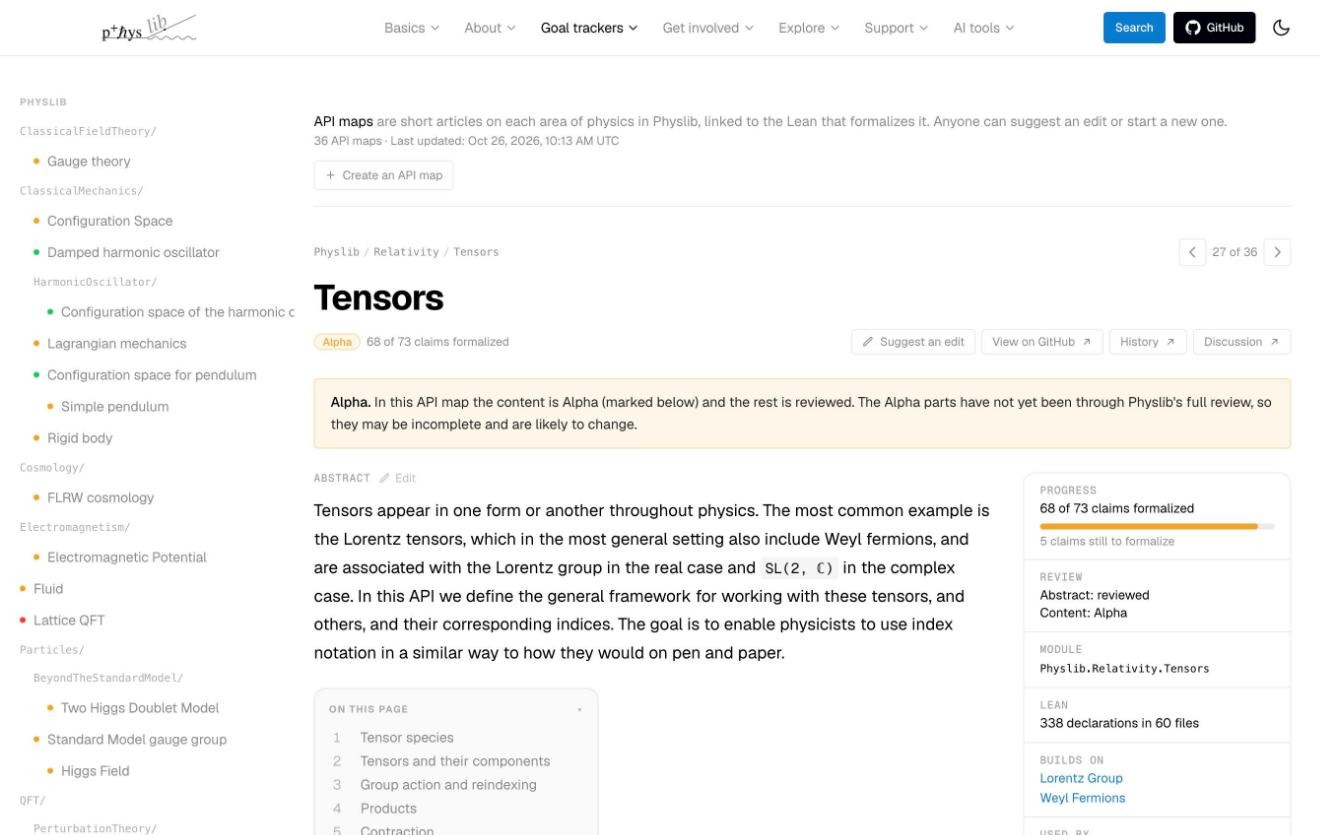
\includegraphics[width=0.97\linewidth]{PhyslibAPIMap.jpg}}}%
    \end{column}
  \end{columns}
  \vfill
\end{frame}

%%%%%%%%%%%%%%%%%%%%%%%%%%%%%%%%%%%%%%%%%%%%%%%%%%%%%%%%%%%%%%%%%%%%%%%%%%%%%%%
%    SECTION 3 -- HOW TO CONTRIBUTE?
%%%%%%%%%%%%%%%%%%%%%%%%%%%%%%%%%%%%%%%%%%%%%%%%%%%%%%%%%%%%%%%%%%%%%%%%%%%%%%%
\begin{jtsection}{3}{How to contribute?}{Contributing}
\end{jtsection}

%%%%%%%%%%%%%%%%%%%%%%%%%%%%%%%%%%%%%%%%%%%%%%%%%%%%%%%%%%%%%%%%%%%%%%%%%%%%%%%
%  3.1  ACTIVITIES ONE COULD DO
%%%%%%%%%%%%%%%%%%%%%%%%%%%%%%%%%%%%%%%%%%%%%%%%%%%%%%%%%%%%%%%%%%%%%%%%%%%%%%%
\begin{frame}{Activities one could do}
  \vfill
  \begin{columns}[T,onlytextwidth]
    \begin{column}{0.48\textwidth}
      \jtroleex{actrowa}{Review}{e.g.\ reviewing PRs in your area.}
      \jtroleex{actrowb}{Refactoring}{e.g.\ refactoring tensors for index
        notation.}
      \jtroleex{actrowc}{Formalization}{e.g.\ extending the formalization of
        invariance of the SM.}
    \end{column}
    \begin{column}{0.48\textwidth}
      \jtroleex{actrowa}{Maintenance}{e.g.\ adding new skills, linters, etc.}
      \jtroleex{actrowb}{Foundational work}{e.g.\ foundations of string theory.}
      \jtroleex{actrowc}{Documentation}{e.g.\ helping add an Atlas in your
        area of expertise.}
    \end{column}
  \end{columns}
  \vfill
\end{frame}

%%%%%%%%%%%%%%%%%%%%%%%%%%%%%%%%%%%%%%%%%%%%%%%%%%%%%%%%%%%%%%%%%%%%%%%%%%%%%%%
%  3.2  CREDIT FOR CONTRIBUTIONS
%  Screenshot is ../Images/FormalContributions.jpg, taken 2 November 2026;
%  re-capture before the talk, the report list drifts.
%%%%%%%%%%%%%%%%%%%%%%%%%%%%%%%%%%%%%%%%%%%%%%%%%%%%%%%%%%%%%%%%%%%%%%%%%%%%%%%
\begin{frame}{Credit for contributions}
  \vfill
  \centering
  {\fontsize{23}{27}\selectfont\bfseries
    \href{https://formalcontributions.com}{%
      \color{jttealink}formalcontributions.com}\par}
  \vspace{8pt}
  \href{https://formalcontributions.com}{%
    \fcolorbox{jtrule}{white}{%
      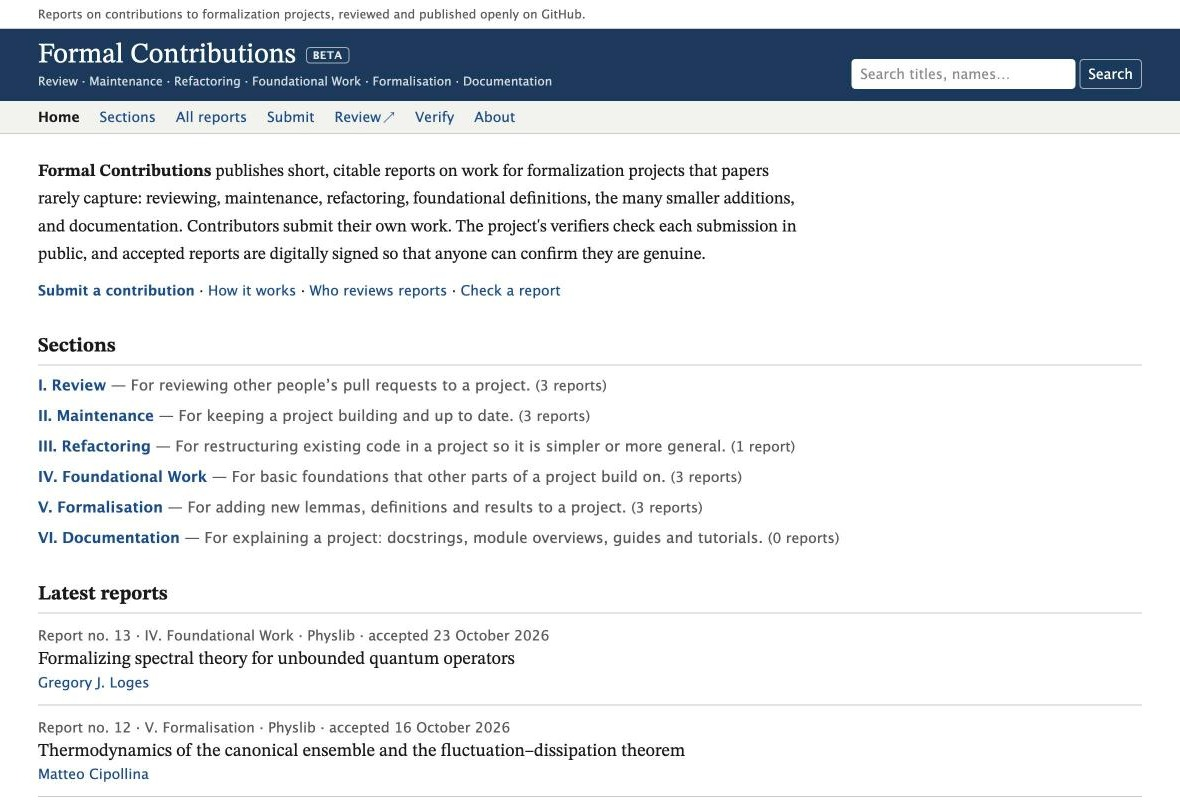
\includegraphics[height=4.7cm]{FormalContributions.jpg}}}%
  \par
  \vfill
\end{frame}

%%%%%%%%%%%%%%%%%%%%%%%%%%%%%%%%%%%%%%%%%%%%%%%%%%%%%%%%%%%%%%%%%%%%%%%%%%%%%%%
%  3.3  PHYSICS 2.0
%%%%%%%%%%%%%%%%%%%%%%%%%%%%%%%%%%%%%%%%%%%%%%%%%%%%%%%%%%%%%%%%%%%%%%%%%%%%%%%
\begin{frame}{Physics 2.0}
  \vfill
  {\color{jttealink}\rule{2.4cm}{1.8pt}}\par
  \vspace{6pt}
  {\fontsize{20}{24}\selectfont\bfseries\color{jtslate}
    A plan for the future of physics\par}
  \vspace{8pt}
  \begin{jtquote}[top=10pt,bottom=10pt]{jttealink}
    {\fontsize{16}{22}\selectfont\color{jtslate}%
      Contributions to projects like {\bfseries Physlib}, with credit given
      from sites like {\bfseries formalcontributions.com}, could make a
      {\bfseries new landscape} for how we do physics.\par}
  \end{jtquote}
  \vfill
\end{frame}

%%%%%%%%%%%%%%%%%%%%%%%%%%%%%%%%%%%%%%%%%%%%%%%%%%%%%%%%%%%%%%%%%%%%%%%%%%%%%%%
%    THANK YOU
%%%%%%%%%%%%%%%%%%%%%%%%%%%%%%%%%%%%%%%%%%%%%%%%%%%%%%%%%%%%%%%%%%%%%%%%%%%%%%%
{
\setbeamertemplate{background}{\jtBackgroundDark}
\setbeamertemplate{footline}{}
\begin{frame}[plain]
  \vfill
  \begin{columns}[T,onlytextwidth]
    \begin{column}{0.97\textwidth}
      {\color{jtondarka}\rule{3.2cm}{2pt}}\par
      \vspace{18pt}

      {\color{jtondark}\fontsize{30}{35}\selectfont\bfseries
        Thank you\par}
      \vspace{10pt}
      {\color{jtondarkm}\fontsize{17}{22}\selectfont
        Happy to discuss how we can make this project better serve the
        needs of the community\par}

      \vspace{24pt}
      {\color{jtondarkm}\rule{\linewidth}{0.5pt}}\par
      \vspace{12pt}

      {\color{jtondark}\fontsize{13}{16}\selectfont\bfseries Joseph Tooby-Smith\par}
      \vspace{4pt}
      {\color{jtondarkm}\jtmeta University of Bath\par}

      \vspace{14pt}
      {\color{jtondarkm}\jtmeta
        \href{https://github.com/leanprover-community/physlib}{%
          \color{jtondarkm}github.com/leanprover-community/physlib}
        \qquad
        \href{https://formalcontributions.com}{%
          \color{jtondarkm}formalcontributions.com}
        \qquad
        \href{https://josephtoobysmith.com/}{%
          \color{jtondarkm}josephtoobysmith.com}\par}
    \end{column}
  \end{columns}
  \vfill
\end{frame}
}

\end{document}
